\documentclass[xcolor={dvipsnames}]{beamer}
\usepackage{HECbeamer}
%  \usepackage{pgfpages}
%  \pgfpagesuselayout{4 on 1}[letterpaper,landscape, border shrink=5mm]
% \usepackage{listings}
% \usepackage{minted}
% \usemintedstyle{vs}
% \newcommand{\saskeyword}[1]{\textcolor{blue}{#1}}
% \newenvironment{sasminted}{\VerbatimEnvironment\begin{minted}[escapeinside=||,fontsize=\small,baselinestretch=1, samepage=true]{sas}}
%  {\end{minted}}

\uselanguage{French}
\languagepath{French}
\title[\color{white}{MATH60604 \S~2f - Prédictions du modèle linéaire}]{MATH60604 \\Modélisation statistique \\ \S~2f - Prédictions du modèle linéaire}
\author{}
\date{\today}
\institute{HEC Montréal\\
Département de sciences de la décision}
\date{} 

\begin{document}
\frame{\titlepage}

\begin{frame}
\frametitle{Valeurs ajustées et prédictions}
\bi
\item En commercialisation par base de données, le but
premier est de développer un modèle pour pouvoir obtenir des prévisions
de la variable dépendante et ensuite prendre des décisions d’affaires basées
sur elles.
\item 
Par exemple, on pourrait vouloir prévoir le montant d’argent dépensé si on
envoie une offre à un client.
\item La procédure habituelle consiste alors à envoyer l’offre à un échantillon de clients, à développer un modèle avec des données, et ensuite à appliquer ce modèle (obtenir les prédictions) pour les autres clients dans la base de
données.
\ei
\end{frame}



\begin{frame}
\frametitle{Prédiction}
\bi
\item On veut estimer la \alert{moyenne de $Y$} quand $\mathbf{X}=\bs{x}$,
\begin{align*}
\E{Y\mid \mathbf{X}=\bs{x}}=\beta_0+\beta_1x_1 + \cdots + \beta_px_p.\end{align*}
\item On pourrait également vouloir \alert{prédire la valeur} d'une nouvelle valeur de la réponse $Y_i$ quand $\mathbf{X}_i=\bs{x}$; on rappelle que
\begin{align*}
Y_i=\beta_0+\beta_1x_1 + \cdots + \beta_px_p +\varepsilon_i.
\end{align*}
\item Que l'on veuille estimer la \alert{moyenne} ou prédire la \alert{valeur} de $Y$ quand $\mathbf{X}=\bs{x}$, les valeurs prédites et ajustées sont égales aux points sur la ``droite'' correspondant à $\mathbf{X}=\bs{x}$,
\begin{align*}
\hat{\beta}_0+\hat{\beta}_1x_{1} + \cdots + \hat{\beta}_px_{p}.
\end{align*}

\ei
% TODO: LEFTOVERS
\end{frame}
\begin{frame}
\frametitle{Davantage d'incertitude pour les prédictions individuelles}
\bi 
\item La moyenne estimée et la prédiction pour un individu sont \textbf{identiques} pour la régression linéaire.
\bi \item nous verrons que ce n'est pas le cas dans les modèles mixtes, dans lesquels on inclut des effets aléatoires pour des individus ou des groupes.
\ei
\item Une fois qu'on a obtenu des estimés des paramètres, on peut obtenir les valeurs ajustées et les prédictions pour
$Y$ pour un ensemble de variables explicatives $\mathrm{X}_1=x_1, \ldots,\mathrm{X}_p=x_p$
\begin{align*}
\hat{Y}=\hat{\beta}_0 +\hat{\beta}_1 x_1+\ldots+\hat{\beta}_px_p.
\end{align*}
\ei
\end{frame}

\begin{frame}
\frametitle{Même prédiction, différentes incertitudes}
\bi \item
 Bien que l'estimateur de la moyenne de $Y$, $\E{Y \mid \mathbf{X}}$, soit identique, cet estimateur sera \alert{\textbf{plus précis}} que la valeur prédite d'une nouvelle variable réponse $Y_i$.
\item L'\textbf{intervalle de confiance} (pour l'espérance) est plus petit que l'\textbf{intervalle de prédiction}.
\bi \item \textbf{explication}: une nouvelle observation inclut un terme d'erreur additionnel $\eps$ qui augmente l'incertitude.
\ei
 \ei
\end{frame}

\begin{frame}[fragile]
\frametitle{Valeurs ajustées et intervalles de confiance pour prédictions en \SASlang}
\bi
\item On crée un nouveau jeu de données \code{newdata} contenant les valeurs des combinaisons de variables explicatives pour lesquelles on veut obtenir des prédictions. 
\item Nous utilisons à titre d'exemple la première observation du jeu de données et on copie la combinaison des valeurs explicatives, mais en faisant varier le temps de fixation de $0$ à $6$ secondes.
\ei
\begin{tcolorbox}[colback=white, colframe=hecblue, title=Code \SASlang pour créer un nouveau jeu de données]
\begin{verbatim}
data newdata;
   set modstat.intention(obs=1);
   do fixation=0 to 6;
      output;
   end;
run;
\end{verbatim}
\end{tcolorbox}
\end{frame}

\begin{frame}[fragile]
\frametitle{Sauvegarder la sortie du modèle linéaire}
\bi
\item Par la suite, on ajuste le modèle linéaire et on sauvegarde l'information dans un objet, disons \code{modelinfo}, afin de faire des prédiction.
\ei
\begin{tcolorbox}[colback=white, colframe=hecblue, title=Code \SASlang pour enregistrer la sortie du modèle linéaire]
\begin{verbatim}
proc glm data=modstat.intention noprint;
class sexe educ revenu;
model intention= fixation emotion 
    sexe age revenu educ / ss3 solution;
store modelinfo; 
run;
\end{verbatim}
\end{tcolorbox}
\end{frame}

\begin{frame}
\frametitle{Prédiction à partie de la sortie}
\bi 
 \item La procédure \code{plm} permet d'obtenir les prédictions pour le modèle spécifié par  \code{modelinfo}. Ces prédictions sont enregistrées dans le fichier temporaire \code{prediction}.
\item On inclut l'intervalle de confiance ponctuel pour la moyenne (\code{lclm} et \code{uclm}) et l'intervalle de prédiction pour les valeurs individuelles (\code{lcl} et \code{ucl}).
\ei
\end{frame}

\begin{frame}[fragile]
% \frametitle{Prédiction à partie de la sortie}

\begin{tcolorbox}[colback=white, colframe=hecblue, title=Code \SASlang pour obtenir les prédictions avec \code{plm} ]
{\small 
\begin{verbatim}
proc plm restore=modelinfo; 
score data=newdata out=prediction predicted 
    lclm uclm lcl ucl; 
run;

proc sgplot data=prediction;
band x=fixation upper=ucl lower=lcl / 
        fill transparency=.5 
        legendlabel="individuelle";
band x=fixation upper=uclm lower=lclm / 
        fill transparency=.1 
        legendlabel="moyenne";
series x=fixation y=predicted / 
legendlabel="prédiction";
yaxis label="intention d'achat";
xaxis label="temps de fixation (en secondes)";
run;
\end{verbatim}
}
\end{tcolorbox}
\end{frame}


\begin{frame}[fragile]
\frametitle{Intervalles de confiance pour la moyenne et intervalles de prédiction}
\begin{center}
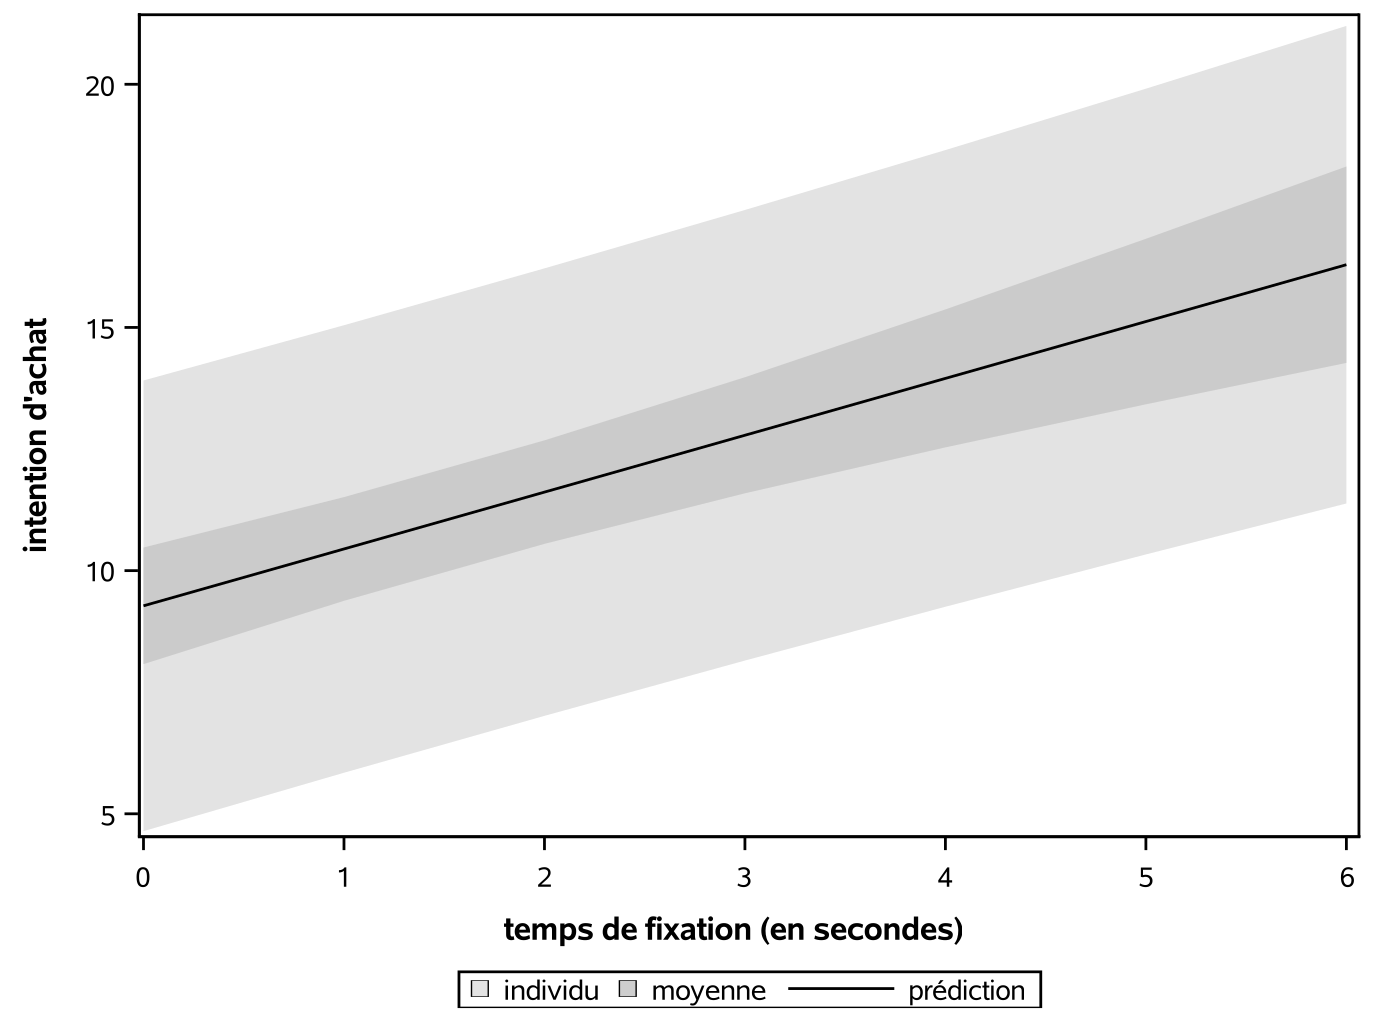
\includegraphics[width = 0.75\linewidth]{img/c2/diapos3-e17}
\end{center}
{\footnotesize L'intervalle de confiance pour la moyenne (gris foncé) est plus étroit que l'intervalle de prédiction (gris clair). Les intervalles de prédiction et de confiance deviennent plus larges à mesure que l'on s'éloigne de la valeur moyenne de \code{fixation}.

}
\end{frame}

\end{document}
